\scanpage{15}
\textcircled{7} Reconstruction of the fundamental I-groupoids $\Pi_1(\mathfrak X';J)$ of $\mathfrak X'$, and of the actions of $\mathcal G'$ on them, in terms of the extension $\unsure{\mathcal E|\Sigma}'$ of $\mathcal G'$ by $\pi_1$, and of the action of $\unsure{\mathcal E|\Sigma}'$ on $\widetilde{\mathfrak X}'(J)$ and $\widetilde{\mathfrak X}'(J)\longrightarrow J$ [and of the maps (7) (8)
\diagram{\begin{tikzcd}[ampersand replacement=\&]
\Psi^{\mathrm{ex}}:\widetilde{\mathfrak X}'(J) \arrow[r] \& \operatorname{Splitt}(\unsure{\mathcal E|\Sigma}'/\mathcal G')/\pi_1
\end{tikzcd}}
\diagram{\begin{tikzcd}[ampersand replacement=\&]
\Psi_{\unsure{j}}:\bigl(\widetilde{\mathfrak X}'(j) \arrow[r,dash] \& \operatorname{Splitt}(\unsure{\mathcal E|\Sigma}'_j/\mathcal G'_j)\bigr)].
\end{tikzcd}}
\margin{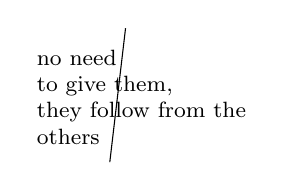
\begin{tikzpicture}[x=1cm,y=1cm]
\node[anchor=north west,align=left,font=\footnotesize] at (0,0) {no need\\to give them,\\they follow from the\\others};
\draw (1.25,0.15) -- (1.05,-1.55);
\end{tikzpicture}}
\[
\operatorname{Ob}\Pi_1=J
\]
\deleted{\unsure{Let} $j,j'\in J$}

\uline{NB} if $\widetilde\xi\in\widetilde{\mathfrak X}'(J)$, $\widetilde{\mathfrak X}'[j]$ (universal covering of $\mathfrak X'$ at $j$) is identified with $\widetilde{\mathfrak X}'$ (since $\widetilde\xi$ is a marked poin\textsuperscript{t} of $\widetilde{\mathfrak X}'$ over $j$
\diagram{\begin{tikzcd}[ampersand replacement=\&]
\widetilde{\mathfrak X}' \arrow[r,"\unsure{\varphi|\psi}_{\widetilde\xi}"] \& \widetilde{\mathfrak X}'[j]
\end{tikzcd}}
If $\gamma\in\pi_1$, we shall have
\[
\Psi_{\gamma\cdot\widetilde\xi}=\Psi_{\widetilde\xi}\circ\gamma_{\widetilde{\mathfrak X}'}^{\deleted{\unsure{-1}}}
\]
so one can say, independently of the choice of the base poin\textsuperscript{t} $\widetilde\xi$
\diagram{\begin{tikzcd}[ampersand replacement=\&]
\widetilde{\mathfrak X}'[j] \& 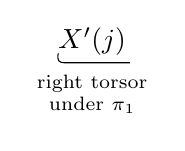
\begin{tikzpicture}[baseline=(torsorfactor.base),x=1cm,y=1cm]
\node[inner sep=0pt] (torsorfactor) at (0,0) {$\mathfrak X'(j)$};
\draw (-0.43,-0.15) .. controls (-0.45,-0.24) and (-0.42,-0.27) .. (-0.35,-0.27) -- (0.48,-0.27);
\node[anchor=north,align=center,font=\scriptsize] at (0,-0.30) {right torsor\\under $\pi_1$};
\end{tikzpicture}\mathbin{\wedge}_{\pi_1}\widetilde{\mathfrak X}' \arrow[l,"\sim"']
\end{tikzcd}}
\mspage{14}
